\documentclass[10pt,a4paper]{article}

\usepackage[a4paper,top=9.5mm,bottom=9.5mm,left=12mm,right=12mm]{geometry}
\usepackage[T1]{fontenc}
\usepackage[default]{lato}
\usepackage{microtype}
\usepackage{xcolor}
\usepackage{graphicx}
\graphicspath{{./}{public/}{../public/}}
\usepackage{tikz}
\usepackage{tabularx}
\usepackage{array}
\usepackage{enumitem}
\usepackage{titlesec}
\usepackage{hyperref}
\usepackage{ragged2e}
\usepackage{setspace}
\usepackage{fancyhdr}

\definecolor{Navy}{HTML}{17324D}
\definecolor{Teal}{HTML}{0F7182}
\definecolor{Ink}{HTML}{17202A}
\definecolor{Muted}{HTML}{5D6773}
\definecolor{Rule}{HTML}{D6DEE5}
\definecolor{Soft}{HTML}{EEF4F7}
\definecolor{SoftTeal}{HTML}{E7F1F2}

\hypersetup{
  colorlinks=true,
  urlcolor=Teal,
  linkcolor=Navy,
  pdfauthor={Jia-Hao Ji},
  pdftitle={Jia-Hao Ji - One-Page Research CV},
  pdfsubject={Biomedical AI, spatial omics, and multi-agent reasoning},
  pdfkeywords={biomedical AI, agentic AI, spatial omics, multi-agent systems, neuroscience}
}
\urlstyle{same}

\pagestyle{fancy}
\fancyhf{}
\renewcommand{\headrulewidth}{0pt}
\renewcommand{\footrulewidth}{0pt}
\fancyfoot[L]{\fontsize{7.5}{8.5}\selectfont\color{Muted}Jia-Hao Ji \textbar{} One-Page Research CV}
\fancyfoot[R]{\fontsize{7.5}{8.5}\selectfont\color{Muted}Updated September 2026}
\setlength{\footskip}{5.8mm}

\setlength{\parindent}{0pt}
\setlength{\parskip}{0pt}
\setstretch{1.00}
\emergencystretch=1em
\hyphenpenalty=10000
\exhyphenpenalty=10000
\tolerance=2500
\color{Ink}

\titleformat{\section}
  {\fontsize{11.6}{12.8}\selectfont\bfseries\color{Navy}}
  {}{0pt}{}
  [\vspace{-0.32em}\color{Rule}\titlerule]
\titlespacing*{\section}{0pt}{0.50em}{0.30em}

\newcommand{\contactsep}{\hspace{0.42em}\textcolor{Rule}{\textbullet}\hspace{0.42em}}
\newcommand{\sidehead}[1]{%
  \vspace{0.50em}%
  {\fontsize{9.8}{10.8}\selectfont\bfseries\color{Navy}#1}\par
  \vspace{0.12em}\color{Rule}\rule{\linewidth}{0.45pt}\color{Ink}\vspace{0.20em}
}
\newcommand{\sidetitle}[1]{{\fontsize{8.95}{10.35}\selectfont\bfseries\color{Ink}#1}}
\newcommand{\sidebody}[1]{{\fontsize{8.65}{10.3}\selectfont\color{Muted}\RaggedRight #1}}
\newcommand{\sideitem}[1]{\item {\fontsize{8.55}{10.15}\selectfont\RaggedRight #1}}
\newenvironment{sideitems}{%
  \begin{itemize}[leftmargin=1.05em,itemsep=0.12em,topsep=0.20em,parsep=0pt,partopsep=0pt,label=\textcolor{Teal}{\raisebox{0.14ex}{\tiny\textbullet}}]
}{\end{itemize}}
\newcommand{\tag}[1]{\colorbox{SoftTeal}{\strut\hspace{0.28em}\textcolor{Navy}{\fontsize{7.7}{8.6}\selectfont\bfseries #1}\hspace{0.28em}}}

\newcommand{\pubtitle}[1]{{\fontsize{9.65}{11.0}\selectfont\bfseries\color{Ink}#1}}
\newcommand{\pubmeta}[1]{{\fontsize{8.35}{9.85}\selectfont\color{Muted}\RaggedRight #1}}
\newcommand{\pubimpact}[1]{{\fontsize{8.65}{10.25}\selectfont\RaggedRight #1}}
\newcommand{\roleline}[3]{%
  \begin{tabularx}{\linewidth}{@{}>{\RaggedRight\arraybackslash}X>{\RaggedLeft\arraybackslash}p{28mm}@{}}
    {\fontsize{9.35}{10.55}\selectfont\bfseries #1} & {\fontsize{8.25}{9.45}\selectfont\color{Muted}#3}\\[-0.12em]
    {\fontsize{8.6}{9.85}\selectfont\color{Teal}#2} &
  \end{tabularx}
}
\newcommand{\cvitem}[1]{\item {\fontsize{8.65}{10.25}\selectfont\RaggedRight #1}}
\newenvironment{cvitems}{%
  \begin{itemize}[leftmargin=1.08em,itemsep=0.10em,topsep=0.20em,parsep=0pt,partopsep=0pt,label=\textcolor{Teal}{\raisebox{0.14ex}{\tiny\textbullet}}]
}{\end{itemize}}

\newcommand{\profilephoto}{%
  \begin{tikzpicture}[baseline=(current bounding box.center)]
    \clip (0,0) circle (15.7mm);
    \node at (0,-0.7mm) {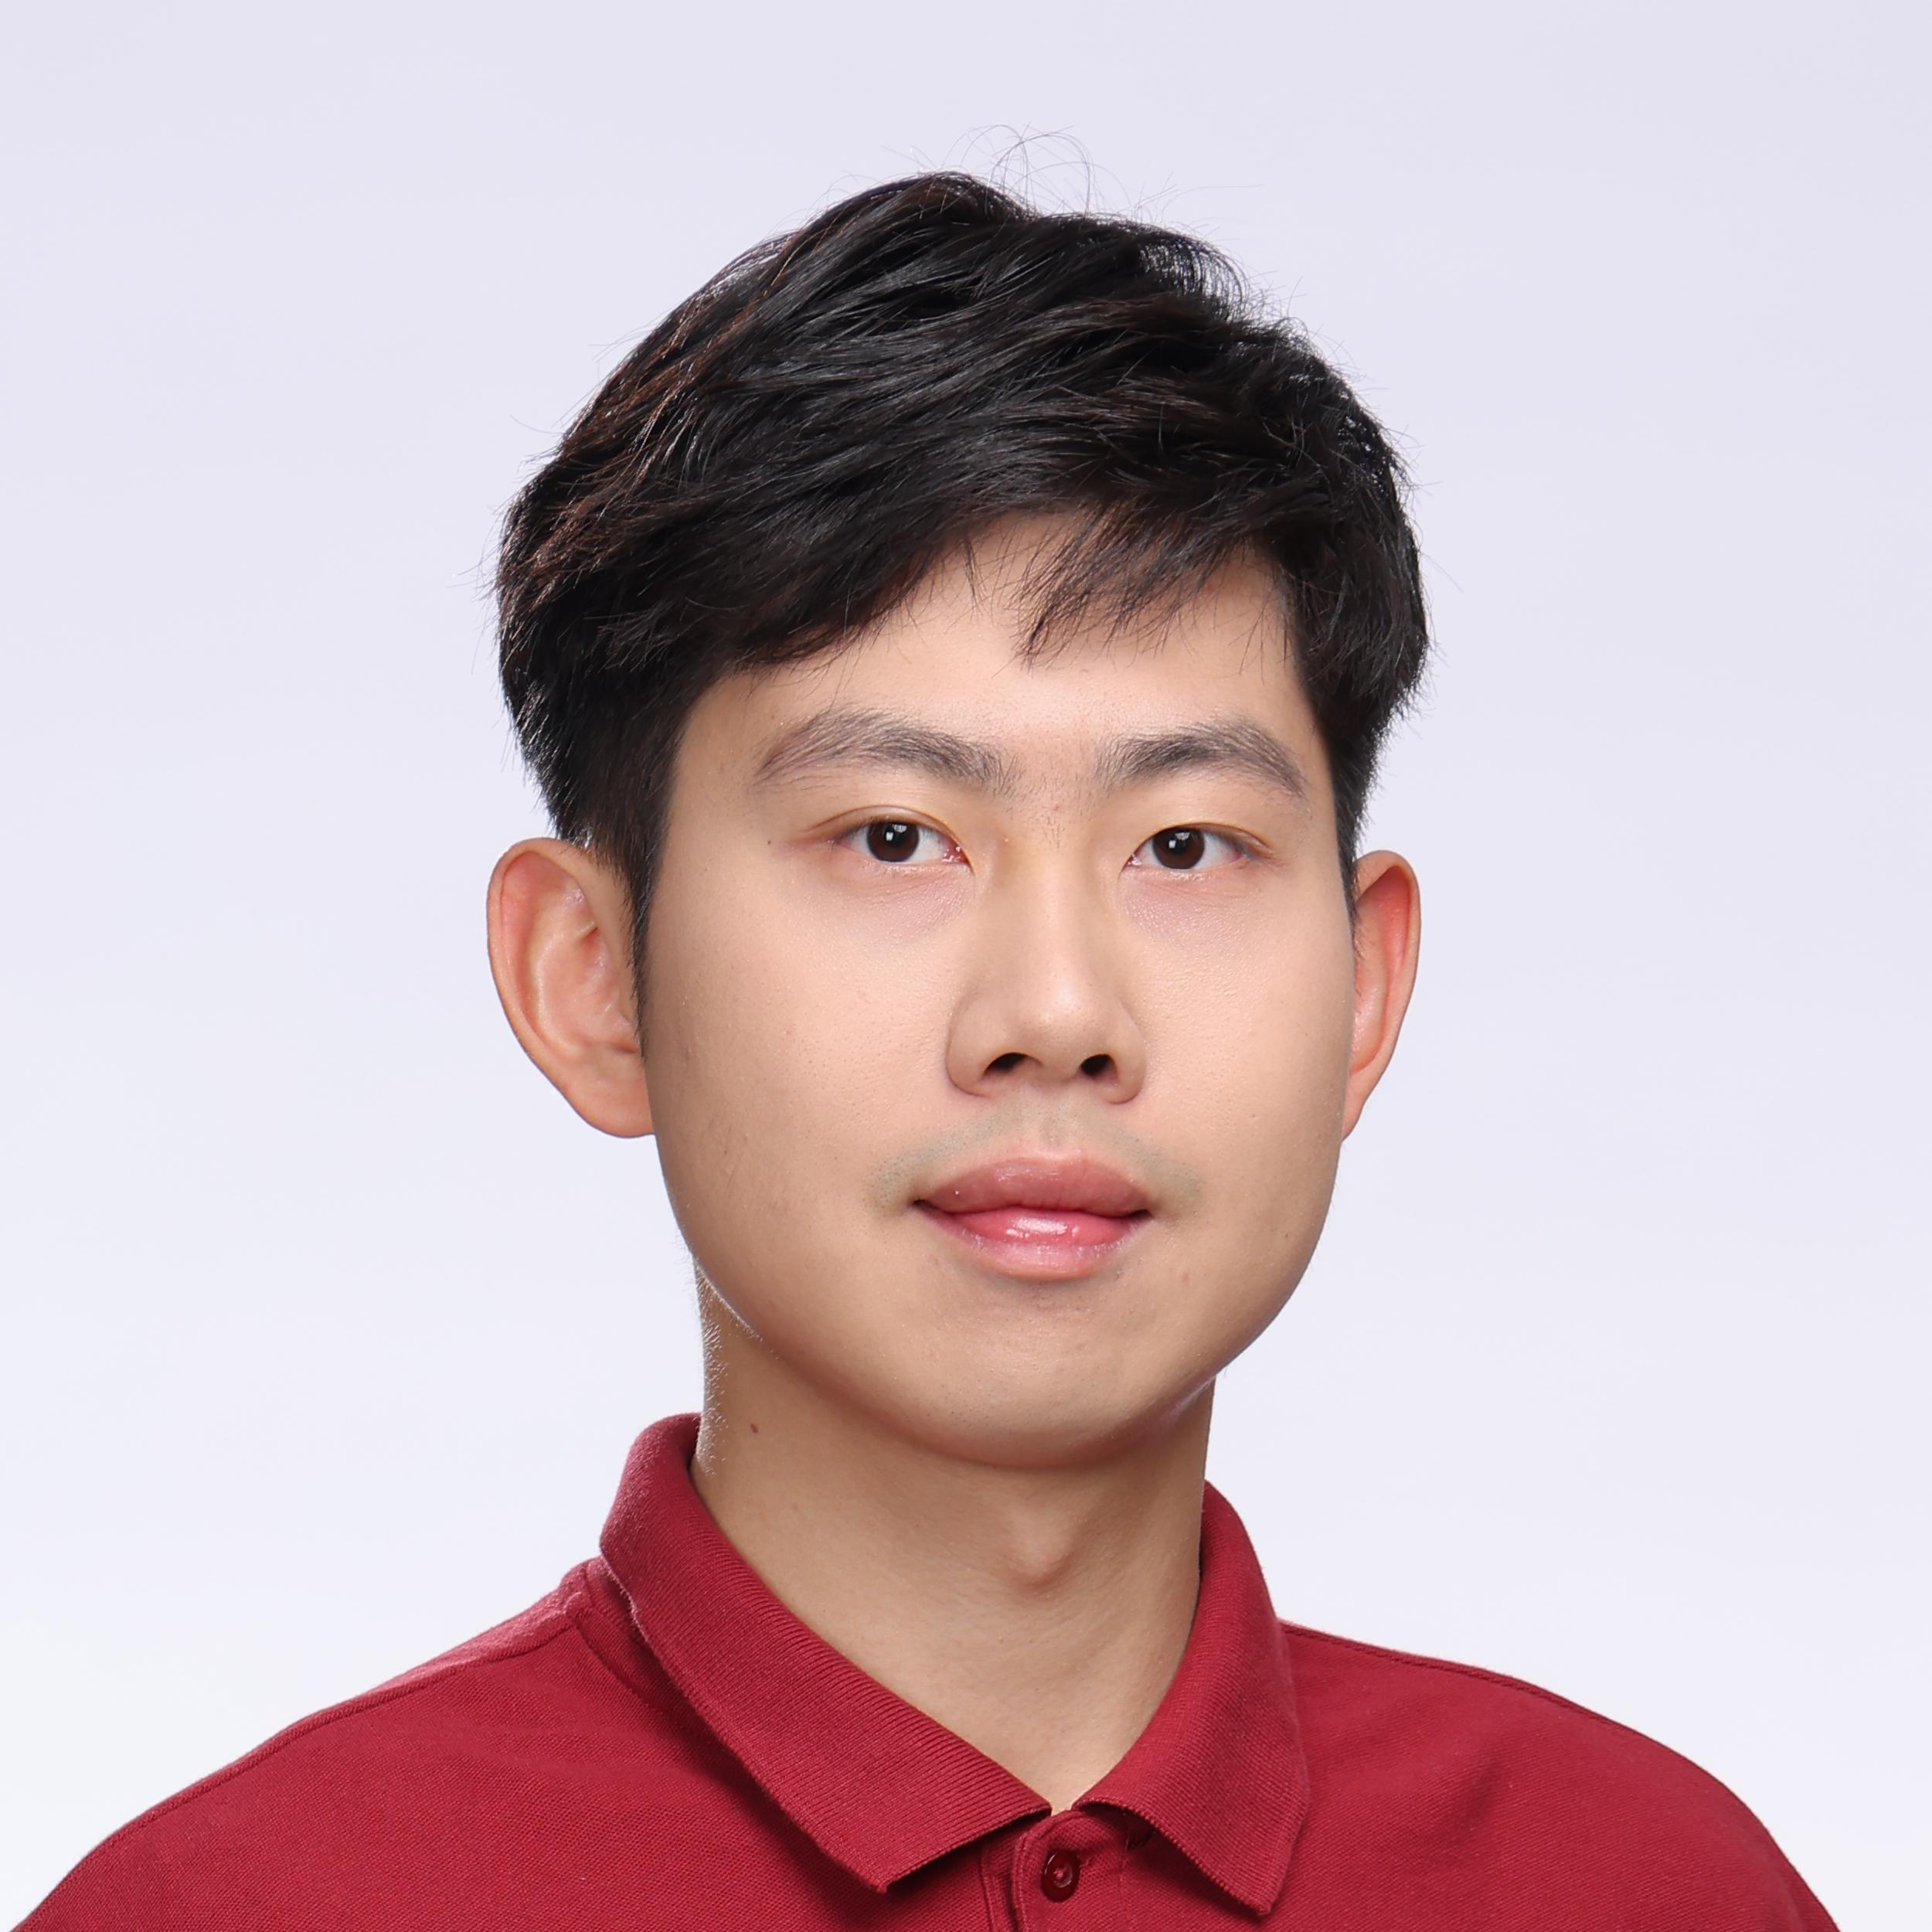
\includegraphics[width=33.5mm]{avatar.jpg}};
    \draw[Teal,line width=0.9pt] (0,0) circle (15.7mm);
  \end{tikzpicture}%
}

\begin{document}

% Header
\noindent\color{Navy}\rule{\textwidth}{2.2pt}\color{Ink}
\vspace{0.34em}

\noindent
\begin{minipage}[t]{0.785\textwidth}
  \vspace{0pt}
  {\fontsize{25.5}{27.5}\selectfont\bfseries\color{Ink}Jia-Hao (Jay) Ji}\par
  \vspace{0.08em}
  {\fontsize{11.1}{12.4}\selectfont\bfseries\color{Navy}M.D. Candidate \textbar{} AI Researcher \textbar{} Physician-Scientist in Training}\par
  \vspace{0.36em}
  {\fontsize{8.85}{10.45}\selectfont\color{Muted}\RaggedRight
    Building reliable agentic and multimodal AI systems for biomedical discovery, with current work in spatial omics, neuroscience, and multi-agent reasoning.
  }\par
  \vspace{0.46em}
  {\fontsize{8.15}{9.3}\selectfont\color{Muted}
    Shanghai, China
    \contactsep \href{mailto:jhji19@fudan.edu.cn}{jhji19@fudan.edu.cn}
    \contactsep \href{https://jiahaoblog.com}{jiahaoblog.com}
    \contactsep \href{https://github.com/Biogod2020}{GitHub}
    \contactsep \href{https://orcid.org/0009-0007-4647-522X}{ORCID}
  }\par
\end{minipage}
\hfill
\begin{minipage}[t]{0.185\textwidth}
  \vspace{0pt}
  \centering\profilephoto
\end{minipage}

\vspace{0.25em}
\color{Rule}\rule{\textwidth}{0.6pt}\color{Ink}
\vspace{0.28em}

% Two-column body
\noindent
\begin{minipage}[t]{0.315\textwidth}
\vspace{0pt}
\RaggedRight

\sidehead{Education}
\sidetitle{Shanghai Medical College, Fudan University}\par
\sidebody{M.D., Eight-Year Clinical Medicine Program}\par
\sidebody{2019--2027 (expected)}\par
\vspace{0.26em}
\sidetitle{University of California, Los Angeles}\par
\sidebody{International Exchange Program, 2021--2022}\par
\vspace{0.26em}
\sidetitle{HKU Queen Mary Hospital}\par
\sidebody{Clinical Elective, Department of Medicine, 2025}\par

\sidehead{Technical Expertise}
\sidetitle{Artificial Intelligence}\par
\sidebody{PyTorch; transformers, GNNs, contrastive learning, VLMs, LLM agents, judge-based evaluation, and multi-agent systems.}\par
\vspace{0.30em}
\sidetitle{Biomedical Data}\par
\sidebody{Spatial transcriptomics, scRNA-seq, histopathology, whole-slide imaging, tissue registration, and computational neuroscience.}\par
\vspace{0.30em}
\sidetitle{Engineering}\par
\sidebody{Python, R, TypeScript, Linux, Git, multi-GPU training, HPC, reproducible pipelines, and experiment auditing.}\par

\sidehead{Selected Systems}
\sidetitle{ASSA}\par
\sidebody{Hierarchical-memory agent framework for long-horizon autonomous work. \href{https://github.com/Biogod2020/ASSA}{GitHub}}\par
\vspace{0.30em}
\sidetitle{Spatial-CLIP}\par
\sidebody{Contrastive vision-language learning for histology--spatial transcriptomics alignment. \href{https://github.com/Biogod2020/Spatial-Clip}{GitHub}}\par

\sidehead{Academic Service \& Honours}
\begin{sideitems}
  \sideitem{Invited workshops on AI-native research workflows, Fudan University, 2025.}
  \sideitem{First Prize, National Biology Olympiad (China); ranked 9th in Guangdong Province.}
\end{sideitems}

\sidehead{Languages}
\sidebody{Mandarin, Cantonese, and Teochew (native); English (TOEFL 105); Spanish (basic).}\par
\end{minipage}
\hfill
\begin{minipage}[t]{0.650\textwidth}
\vspace{0pt}
\RaggedRight

\section*{Selected Publications and Manuscripts}

\pubtitle{Candidate supply and answer selection shape the value of LLM judging in multi-agent systems}\par
\pubmeta{\textbf{Jia-Hao Ji}, Sijie Li, Jiabei Cheng, Zixi She, Jin-Tai Yu, and Zhiyuan Yuan. \href{https://arxiv.org/abs/2608.25937}{arXiv:2608.25937}, 2026.}\par
\pubimpact{Separated candidate generation, answer recognition, and terminal selection across five benchmarks. Analysed 15,336 questions and replayed 81,390 fixed candidate pools; changing only final selection increased accuracy from 63.82\% to 70.82--70.95\%.}\par

\vspace{0.30em}
\pubtitle{SpatialDataAgent: Autonomous Spatial Omics Data Curation at Decade Scale}\par
\pubmeta{\textbf{Jia-Hao Ji}, Qi Zou, Jiabei Cheng, Zixi She, Yining Hao, Weishi Liu, Daoliang Zhang, Zhikang Wang, Jin-Tai Yu, and Zhiyuan Yuan. \href{https://doi.org/10.64898/2026.05.27.727615}{bioRxiv preprint}, 2026.}\par
\pubimpact{First author and lead developer. Built an evidence-grounded agentic workflow that recovered 769 paired H\&E--spatial transcriptomics datasets and assembled HESRT with 29.2 million spots or cells.}\par

\vspace{0.30em}
\pubtitle{Spatiotemporally resolved transcriptome unveils reactive subpallial microglia underlying cholinergic vulnerability in Alzheimer's disease}\par
\pubmeta{\textbf{Jia-Hao Ji} (co-first author) et al. Manuscript, 2026.}\par
\pubimpact{Integrated spatial transcriptomics, single-nucleus sequencing, and in situ amyloid pathology across 12.36 million spatial profiles to characterize microglial microenvironments and cholinergic vulnerability.}\par

\section*{Research Experience}

\roleline{Researcher and Project Lead}{Fudan Data-Driven Future Lab \& Institute of Medical Genetics}{Sep 2023--Present}
\pubmeta{Advisors: Prof. Jin-Tai Yu and Prof. Zhiyuan Yuan \textbar{} Alzheimer's disease, spatial omics, and biomedical AI}\par
\begin{cvitems}
  \cvitem{Lead computational projects spanning large-scale spatial-data curation, multimodal tissue registration, and disease-focused analysis of histology and molecular profiles.}
  \cvitem{Developed transformer-based and image-registration pipelines aligning whole-slide pathology with spatial transcriptomic coordinates and mapping beta-amyloid plaque microenvironments.}
  \cvitem{Designed reproducible agentic workflows with explicit schemas, evidence tracking, failure auditing, and multi-stage validation.}
\end{cvitems}

\vspace{0.18em}
\roleline{Undergraduate Researcher}{Prof. Bin Song's Lab, Fudan University}{Oct 2021--Jun 2023}
\begin{cvitems}
  \cvitem{Built scRNA-seq pipelines to identify markers relevant to the purity, safety, and therapeutic potential of iPSC-derived dopaminergic progenitor transplantation in Parkinson's disease.}
\end{cvitems}

\vspace{0.15em}
\roleline{Undergraduate Researcher}{Prof. Fei Lan's Lab, Institutes of Biomedical Sciences}{Sep 2019--Jul 2021}
\begin{cvitems}
  \cvitem{Conducted wet-lab work in cell culture, molecular assays, DNA methylation, and epigenetic regulation.}
\end{cvitems}

\end{minipage}

\end{document}
